\documentclass[tikz,border=5pt]{standalone}
\usepackage[UTF8]{ctex}
\usepackage{amsmath,amssymb}
\usetikzlibrary{arrows.meta,calc,angles,quotes,decorations.pathmorphing,patterns}
\definecolor{ink}{HTML}{243447}\definecolor{blue}{HTML}{2765A2}
\definecolor{green}{HTML}{3F7D5B}\definecolor{red}{HTML}{B74739}
\tikzset{body/.style={draw=ink,thick},vec/.style={draw=blue,thick,-{Latex}},guide/.style={gray!65,dashed},dim/.style={ink,{Latex}-{Latex}},line cap=round,line join=round}
\begin{document}

\begin{tikzpicture}
\draw[body](0,0)--(0,2)--(5.4,2);\draw[body](0,0)--(5.4,0);
\fill[blue!7](.03,.03)rectangle(2.97,1.97);
\draw[body,fill=gray!15](3,0)rectangle(3.13,2);
\draw[body](3.13,1)--(3.65,1);
\draw[body,decorate,decoration={coil,aspect=.45,segment length=5pt,amplitude=4pt}](3.65,1)--(5.4,1);
\draw[body](5.4,-.25)--(5.4,2.25);
\foreach \y in {-.2,.1,...,2.2}\draw[gray](5.4,\y)--++(.18,.15);
\node at(1.5,1.1){$p,V,T$};\node at(4.3,1.65){$k$};
\node at(4.3,.35){外压 $p_0$};\node[above]at(3.07,2.25){$S_0$};
\draw[vec](3.1,-.7)--(4.6,-.7)node[right]{$q$};
\end{tikzpicture}
\begin{tikzpicture}
\draw[body,fill=gray!12](-.08,-1.5)rectangle(.08,1.5);
\draw[vec](0,.85)--(2.4,.85)node[right]{$pS_0$};
\draw[red,thick,-{Latex}](0,.1)--(-2.4,.1)node[left]{$p_0S_0$};
\draw[green,thick,-{Latex}](0,-.65)--(-1.7,-.65)node[left]{$kq$（$q>0$）};
\draw[vec](-1.5,-2.1)--(1.5,-2.1)node[right]{$+q$};
\draw[red,thick,-{Latex}](0,1.35)--(-1.6,1.35)node[left]{$f_0$（膨胀）};
\draw[vec](0,-1.1)--(1.6,-1.1)node[right]{$f_0$（压缩）};
\end{tikzpicture}
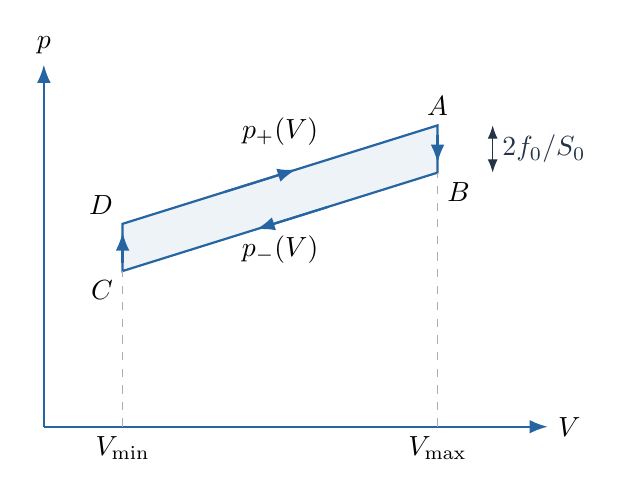
\begin{tikzpicture}
\draw[vec](0,0)--(6.4,0)node[right]{$V$};\draw[vec](0,0)--(0,4.6)node[above]{$p$};
\coordinate(D)at(1,2.577);\coordinate(A)at(5,3.827);\coordinate(B)at(5,3.227);\coordinate(C)at(1,1.977);
\fill[blue!8](D)--(A)--(B)--(C)--cycle;
\draw[blue,thick](D)--(A)--(B)--(C)--cycle;
\draw[vec](2.3,2.983)--(3.2,3.264);
\draw[vec](5,3.7)--(5,3.35);
\draw[vec](3.6,2.789)--(2.7,2.508);
\draw[vec](1,2.08)--(1,2.47);
\node[above]at(A){$A$};\node[below right]at(B){$B$};\node[below left]at(C){$C$};\node[above left]at(D){$D$};
\draw[guide](1,0)--(C);\draw[guide](5,0)--(B);
\node[below]at(1,0){$V_{\min}$};\node[below]at(5,0){$V_{\max}$};
\draw[dim](5.7,3.227)--(5.7,3.827)node[right,midway]{$2f_0/S_0$};
\node[above,sloped]at(3,3.45){$p_+(V)$};\node[below]at(3,2.55){$p_-(V)$};
\end{tikzpicture}
\end{document}
